\chapter{Digital Signal Processing}

Digital signal processing is the basis of computer controlled system, and computer controlled system is an important use case of digital signal processing.

This chapter servers as a brief introduction to digital signal processing, including commonly seen discrete signal and digital system features, $z$-transform and frequency domain analysis of discrete signals and digital systems, signal sampling and reconstruction, discrete Fourier transform and digital filtering.

\section{Motivation}

It has become a common practice nowadays to use digital controllers over analog controllers as the preferable choice in most occasions. A commonly used block diagram of a digital processing system looks like Fig. \ref{fig:digital_system}. The digital and analog modules are given by the black and the red shapes respectively. The analog-to-digital converter (ADC) and the digital-to-analog converter (DAC) bridges the digital and analog worlds, and they are colored in orange.
\begin{figure}
	\centering
	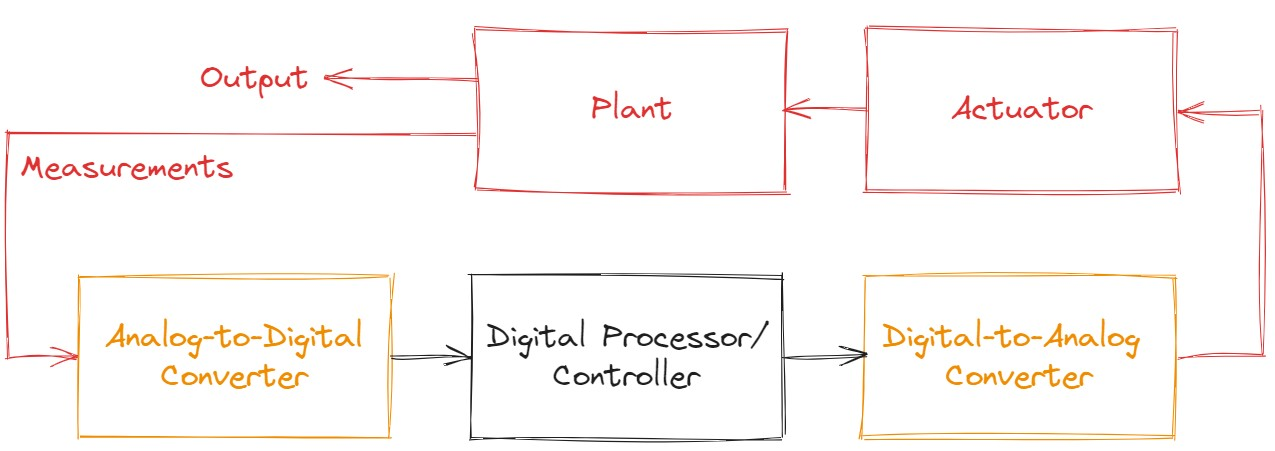
\includegraphics[width=300pt]{chapters/ch-signal-processing/figures/digital_system.jpg}
	\caption{A block diagram of a digital system.} \label{fig:digital_system}
\end{figure}

A digital processing system has the following advantages over a conventional analog processing system.
\begin{itemize}
	\item More flexible. Digital processor is usually re-programmable, thus making it cheaper and faster to add and test new features or functions.
	\item More controllable performance and accuracy. The performance and accuracy of a digital system is more controllable, deterministic and consistent than an analog system.
	\item Easier shareable. The digitized signals and the control algorithm itself can be easily stored and shared. 
\end{itemize}

However, digital system is not always an superior alternative to the counterpart analog system. There are at least the following drawbacks.
\begin{itemize}
	\item More expensive when the function is simple and can be easily realized with an analog circuit. The ADCs, DACs and the digital processor can all introduce additional costs. It is possible that sometimes the function is so simple that it is not worth introducing a digital system.
	\item Slower and has a strict bandwidth requirement. Digital system has been made faster and cheaper in the past years. Nevertheless, there are still tasks where the speed and the bandwidth of a digital system is too slow. In such cases, analog system or optical system might be a better solution.
\end{itemize}

\section{Basic Concepts about Digital Signals and Systems}

Basic concepts and categories of digital signals and systems are introduced.

\subsection{Signals Channel and Dimension}

Signals, both analog and digital, can be scalars of vectors, and it is often formulated as a (vector) function of some independent variables such as time. The length of the vector and the number of independent variables of a digital signal determine the number of channels and the dimensions of the signal.

A signal with vector size $n$ and number of independent variables $m$ is known as a $n$-channel-$m$-dimensional signal. For example, consider a colored image
\begin{eqnarray}
	I(x,y) &=& \left[\begin{array}{c}
		I_r(x,y) \\
		I_g(x,y) \\
		I_b(x,y)
	\end{array}\right] \nonumber
\end{eqnarray}
where $I_r$, $I_g$, $I_b$ and $(x,y)$ are the RGBs and the coordinate of the pixels respectively. This is a 3-channel-2-dimensional signal.

Though multi-channel-multi-dimensional signals are very common, for the convenience of study, the chapter will mostly focus on single-channel-single-dimensional signals.

\subsection{Continuous, Discrete and Digital Signals}

If a signal is continuous in both the time scale (it is defined at any instant of time) and value scale (it has infinite digits of accuracy in its value) is no doubt a continuous signal. Many physical signals, such as the speed of a car, can be modeled by a continuous signal.

Consider sampling a continuous signal by recording its values in countable and discrete timestamps. The signal becomes a discrete-time signal. It is defined only at the sampling timestamps. From value scale vise, it still has infinite digits of accuracy.

Instead of sampling, consider quantizing the signal by mapping its values to a set of discrete values, i.e., usually values with finite digits. The signal becomes a discrete-valued signal. It is defined on a continuous time scale, but the values it can take at any time instant is limited by the digits.

A signal that is both discrete-time and discrete-valued is also known as a digital signal. A demonstrative figure is given in Fig. \ref{fig:signal_types}. 
\begin{figure}
	\centering
	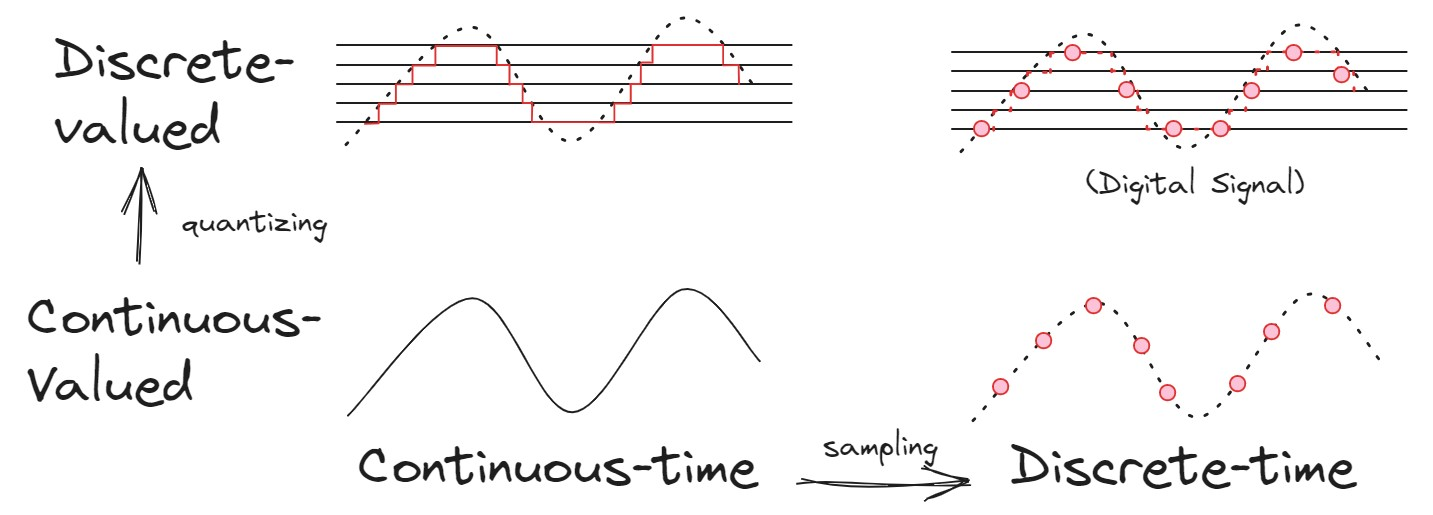
\includegraphics[width=300pt]{chapters/ch-signal-processing/figures/signal_types.jpg}
	\caption{Continuous and discrete signals.} \label{fig:signal_types}
\end{figure}

\subsection{Deterministic and Random Signals}

There is always random noise and stochastic disturbances in a physical system. From this point of view, no system or signal is deterministic. In practice, so long as the signal or system model is to describe the actual signal or system to reasonable accuracy, we would consider the signal or system to be deterministic.

In contrast, if the signal cannot be described by the required reasonable accuracy, or if it simply too complicated to do so, the signal is considered a random signal.

Deterministic signals and models are relatively easier to analyze. When it comes to random signals and stochastic systems, probability and statistics based analysis are usually adopted.

\section{Commonly Seen Digital Signals and Features}

Commonly seen elementary digital signals and their features are introduced. Notice that similar features can be defined for continuous signals as well such as periodic signal, energy and power of signal, etc., but they are not discussed in this section.

\subsection{Elementary signals}

The unit sample sequence is given by
\begin{eqnarray}
	\delta(n) &=& \left\{\begin{array}{cc}
		1 & n = 0 \\
		0 & \textup{otherwise}
	\end{array}\right. \nonumber
\end{eqnarray}
The unit step signal is given by
\begin{eqnarray}
	u(n) &=& \left\{\begin{array}{cc}
		1 & n \geq 0 \\
		0 & \textup{otherwise}
	\end{array}\right. \nonumber
\end{eqnarray}
The unit ramp signal is given by 
\begin{eqnarray}
	u_r(n) &=& \left\{\begin{array}{cc}
		n & n \geq 0 \\
		0 & \textup{otherwise}
	\end{array}\right. \nonumber
\end{eqnarray}
The exponential signal is given by
\begin{eqnarray}
	x(n) &=& a^n \nonumber
\end{eqnarray}
where notice that $a$ can be a complex value denoted by $a=re^{j\theta}$, in which case
\begin{eqnarray}
	x(n) = r^ne^{j\theta n} = r^n\left(\textup{cos}(\theta n) + j\textup{sin}(\theta n)\right) \nonumber
\end{eqnarray}

\subsection{Energy and Power of a Signal}

The energy and power of a signal can be calculated by
\begin{eqnarray}
	E &=& \sum_{n=-\infty}^{\infty} |x(n)|^2 \nonumber \\
	P &=& \lim_{N\rightarrow\infty} \dfrac{1}{2N+1}\sum_{n=-N}^{N}|x(n)|^2 \nonumber
\end{eqnarray}
respectively. The signals whose energy is finite is known as an energy signal. Likewise, the signals with finite power is known as a power signal. From the definition, we know that an energy signal must have a power of $0$. Examples are given in Fig. \ref{fig:energypowersignal}.
\begin{figure}
	\centering
	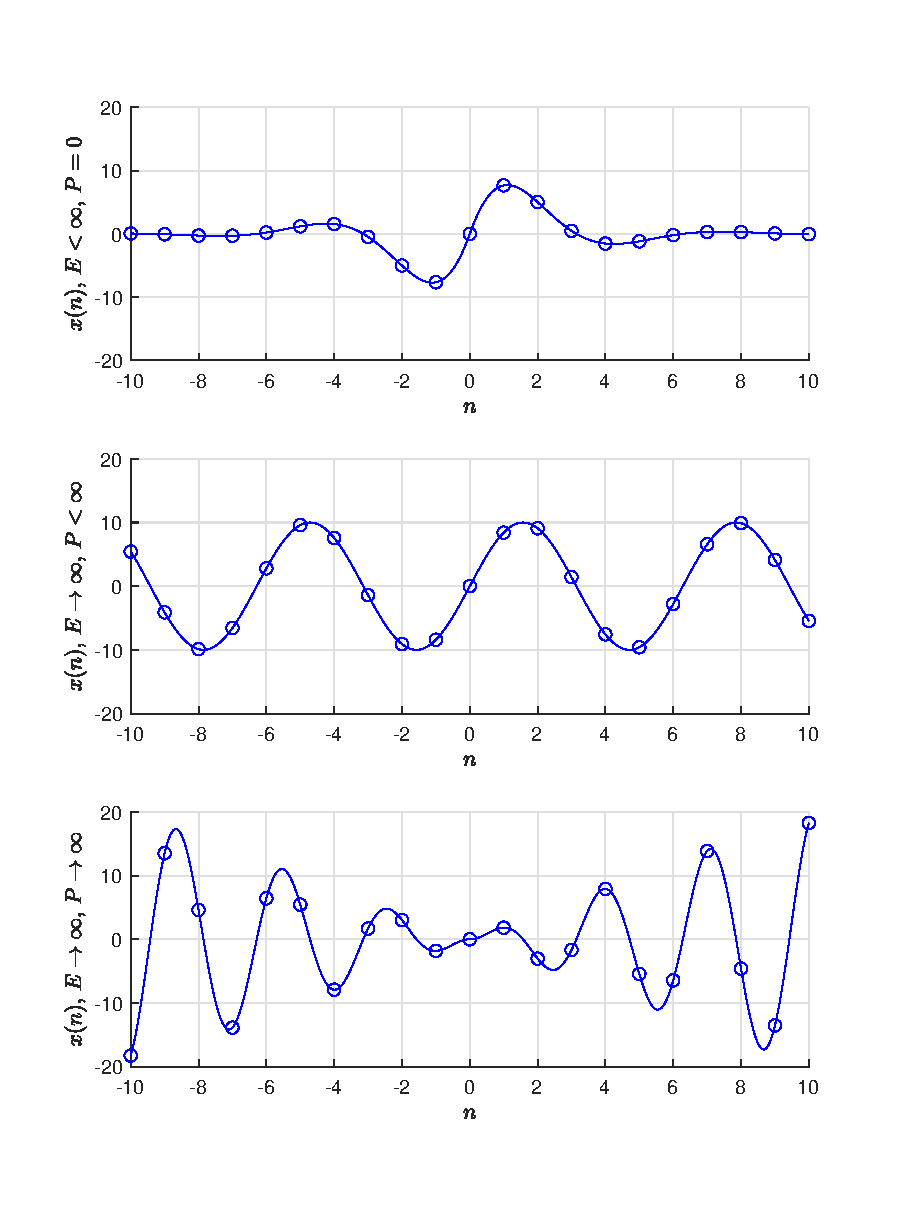
\includegraphics[width=300pt]{chapters/ch-signal-processing/figures/energypowersignal.eps}
	\caption{Example of energy and power signals.} \label{fig:energypowersignal}
\end{figure}

\subsection{Periodic Signal}

A signal $x(n)$ is periodic if
\begin{eqnarray}
	x(n) &=& x(n + N), \textup{~for all~} n \nonumber
\end{eqnarray}
and the smallest $N>0$ is the period of the signal. Notice that a constant signal $x(n)=c$ is often taken as a periodic signal as well, but of non-definable fundamental period. In the remaining of our discussion, we shall consider the ``regular'' periodic signal with $N>0$ unless otherwise emphasized.

It can be proved easily that a period signal has finite power so long as $|x(n)|$ is finite for any timestamp. The energy, on the other hand, is always infinite.

\subsection{Symmetric and Antisymmetric Signals}

A signal $x(n)$ is symmetric (also known as even) if
\begin{eqnarray}
	x(n) &=& x(-n) \nonumber
\end{eqnarray}
A signal $x(n)$ is asymmetric (also known as odd) if
\begin{eqnarray}
	x(n) &=& -x(-n) \nonumber
\end{eqnarray}

Given any signal $x(n)$, define
\begin{eqnarray}
	x_e(n) &=& \dfrac{1}{2}\left[x(n) + x(-n)\right] \nonumber \\
	x_o(n) &=& \dfrac{1}{2}\left[x(n) - x(-n)\right] \nonumber
\end{eqnarray}
It can be easily verified that $x(n) = x_e(n) + x_o(n)$. Therefore, we can conclude that any signal can be decomposed into the symmetric and the antisymmetric portions.

\section{Commonly Seen Operations on a Signal}

For a general discrete signal $x(n)$, $x(-n)$ is a fold of the signal at $n=0$. We can easily prove that $x(-n+2k)$ is a fold of the signal at $n=k$.

Signal $x(n-k)$ is a shift of the original signal $x(n)$ to the right by $k$ samples, i.e., it is $x(n)$ delayed by $k$ samples. Likewise, $x(n+k)$ is the original signal to shift to the left.

Signal $x(\mu n)$, $\mu \in \mathbb{N}^+$ is a time-scaling or down-sampling of the original signal $x(n)$. Graphical wise, it ``squeezes''. A demonstrative figure is given in Fig. \ref{fig:downsampling}. The values captured by the blue circle is the down sampled signal sequence. In this example, $\mu=2$, i.e., one out of two samples are captured.
\begin{figure}
	\centering
	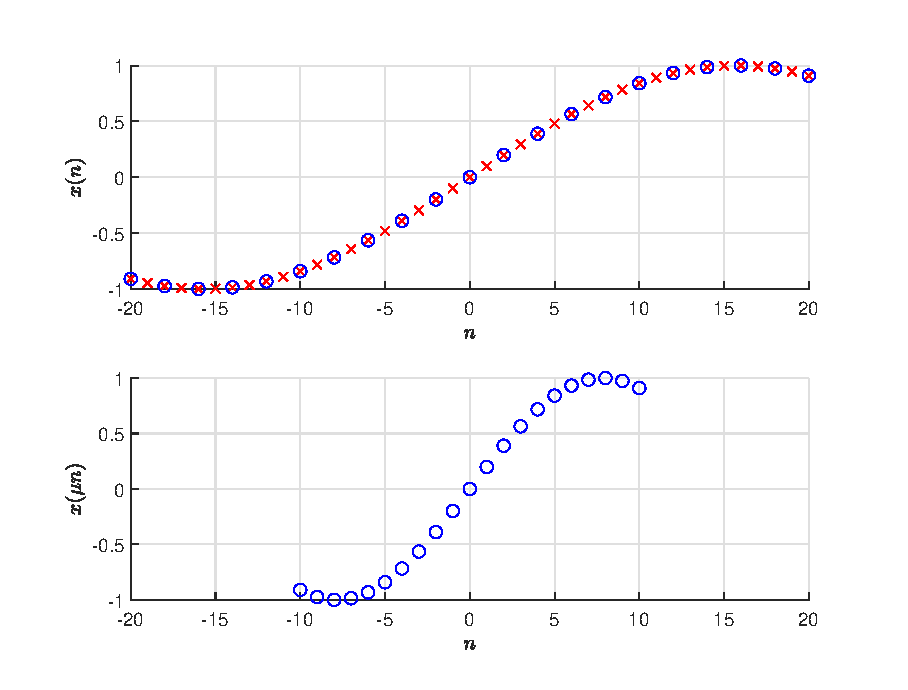
\includegraphics[width=300pt]{chapters/ch-signal-processing/figures/downsampling.eps}
	\caption{A demonstration of down-sampling.} \label{fig:downsampling}
\end{figure}

\section{Digital System}

A digital system maps discrete signal $x(n)$ to another discrete signal $y(n)$. It can be described by
\begin{eqnarray}
	y(n) &=& \mathcal{T}[x(n)] \nonumber
\end{eqnarray}
in general. The system is denoted by $\mathcal{T}$.

\subsection{Input-Output Model}

There are varieties of ways to model the system. A commonly used way is to use an input-output model described by the difference equation. A simple example is given below.
\begin{eqnarray}
	y(k) = \sum_{i=-\infty}^{k-1}x(i) = y(k-1) + x(k-1) \label{eq:diffrenceeqexp}
\end{eqnarray}
Equation \eqref{eq:diffrenceeqexp} calculates the aggregated sum of the input signal. For this system, we can see that its output $y(k)$ can be entirely described by its previous value $y(k-1)$ and the current input $x(k)$. This is because all the ``historical information'' priori to $k-1$ that is useful in calculating $y(k)$ is contained in $y(k-1)$. 

In general, if the current status of a system can be formulated as a function of the one-step previous status of the system and the current input and noise, the system model is known as a \textit{Markov process}. Markov process is widely used in modeling the system behavior. The famous state-space realization of a system is a systematic way of using a Markov process to model a system. 

By tracing back in time, we can find the ``initial state'' of a Markov process. In the context of \eqref{eq:diffrenceeqexp}, initial state can be denoted as $y(0)$. We do not care the values of $y(k)$ and $x(k)$ priori to $k=0$. From the recursive equation \eqref{eq:diffrenceeqexp}, it is obvious that $y(k)$ is essentially determined by the initial state $y(0)$ and the historical inputs $x(0), ..., x(k-1)$.

For the convenience of analysis, it is quite common that zero initial state (also known as relaxed initial state) $y(0)=0$ is assumed, which allows us to focus on the study of input-output relationship. The system response, in which case only affected by the inputs $x(0), ..., x(k-1)$, is known as the \textit{zero state response}. Likewise, there is the \textit{zero input response} of the system where non-zero initial state $y(0)\neq 0$ and zero input $x(k)=0$ are considered.

\subsection{Different Types of Digital Systems} 







\section{Frequency Domain Analysis}


\section{Sampling and Reconstruction of a Signal}

\section{DFT}

\section{Digital Filtering}









